\section{Search Granularity}\label{sec:search_granularity}

If one searched only at the nominal mass points, i.e.\ those defined by the generated MC samples (\cref{fig:ggtt_sample_granularity}), then it is possible that a signal excess at a mass point between nominal mass points could be missed. This is because the analysis categories are designed to target a particular mass point, and could have a selection that is sensitive only to a narrow range of masses around the targeted mass point. The most direct way to understand this is to consider the $m(\ggtt)/\mgg$ variable that is an input to the pNN selection. This distribution is shown in \cref{fig:training_features_7} for simulated background and signal events in the \XTwoHH search. For $\mX=260$\GeV, a highly discriminating cut would be a window around the peak of the signal distribution, however this would almost completely exclude the 500\GeV and 1000\GeV signals also shown in the plot.

In practice, the pNN selection is more complex than this, and there are more nominal mass points than shown in the plot, but the principle remains the same. To ensure that there is good sensitivity to all mass points in the search region, analysis categories are created at intermediate mass points, and the corresponding signals are also searched for. The granularity at which these intermediate mass points are chosen is determined by a procedure that is described in the rest of this section. 

The sensitivity to signals in between nominal mass points is studied by evaluating the expected upper limit for a nominal mass point when using the analysis categories designed for neighbouring mass points. Examples of this in the \XTwoHH search are shown in \cref{fig:limit_granulaity_graviton_changes}. For the $\mX=350$\GeV signal, the categories that are designed for $\mX=350$ lead to the lowest expected upper limit, as expected. However, if using the categories designed for $\mX=320$\GeV, the limit is worse by about 50\%. Assuming that the reduction in sensitivity is linear with the distance in $\mX$ between a signal and a nominal mass point, this suggests that a signal between $\mX=320$ and 350\GeV may have a reduced sensitivity of up to 25\%. By introducing an intermediate mass point at 335\GeV, the maximum reduction in sensitivity to signals in the 320--350\GeV range is estimated to be 12.5\%, or if two points are added at 330 and 340\GeV, the maximum reduction in sensitivity is estimated to be 8.3\%. 

\begin{figure}
  \centering
  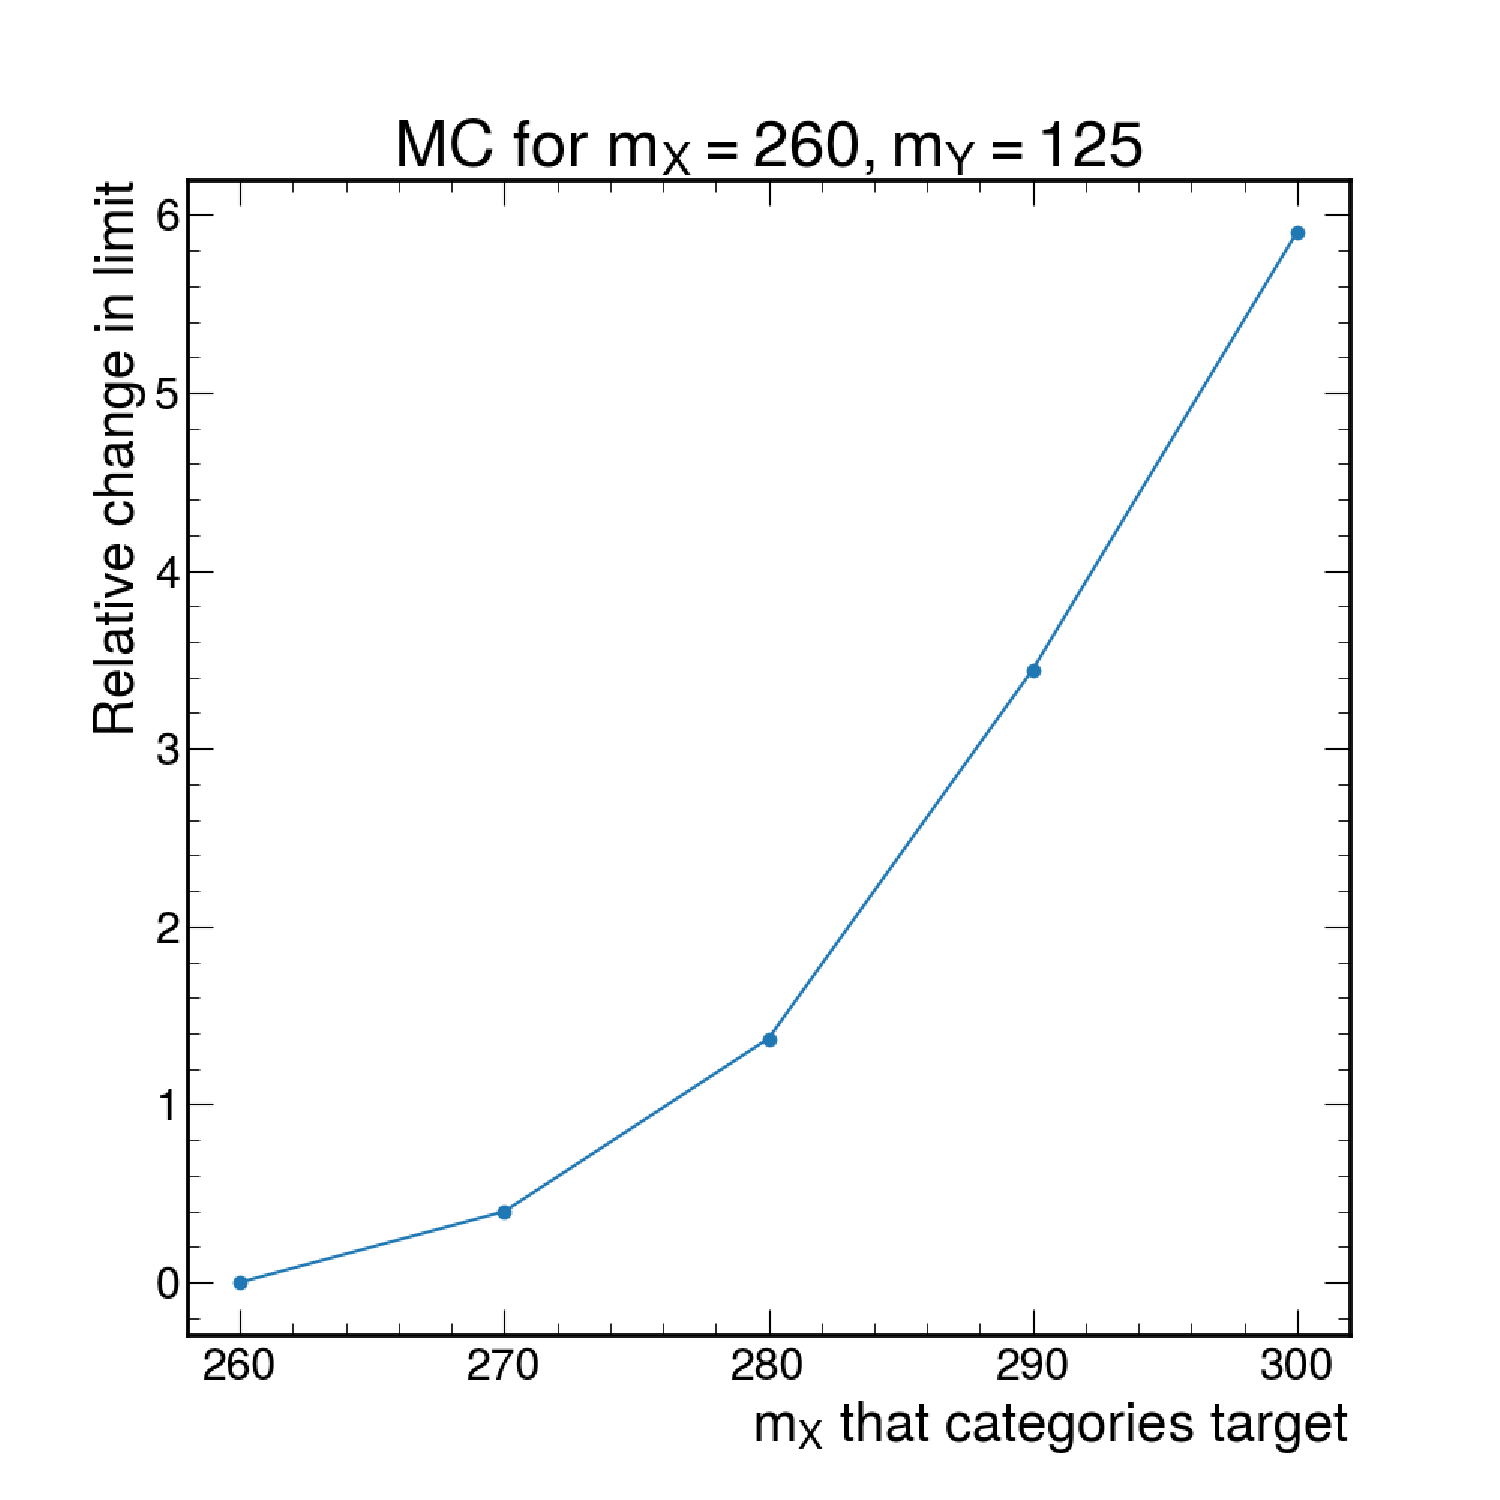
\includegraphics[width=.49\linewidth]{Figures/Dihiggs/results/LimitGranularity/Graviton/mx_260_my_125_mx.pdf}
  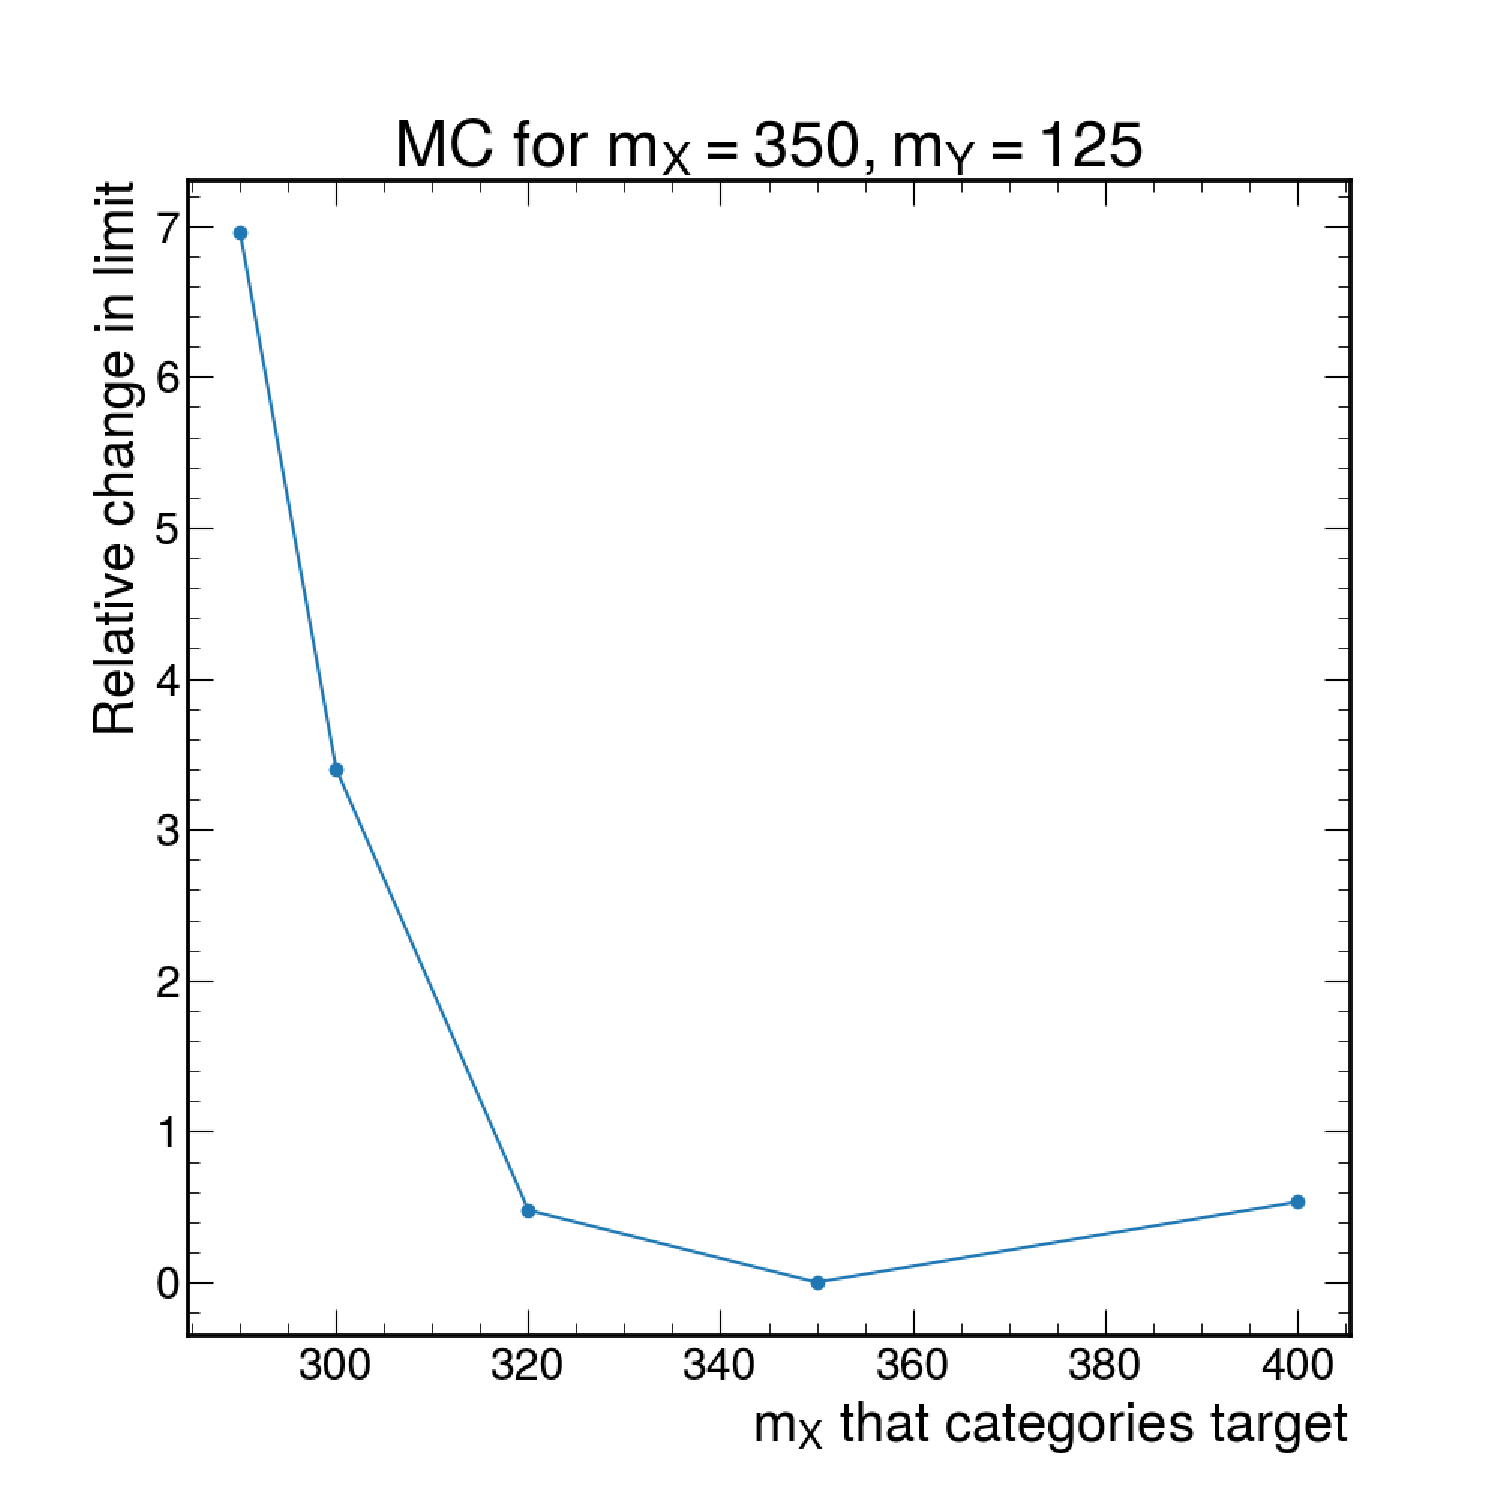
\includegraphics[width=.49\linewidth]{Figures/Dihiggs/results/LimitGranularity/Graviton/mx_350_my_125_mx.pdf} \\
  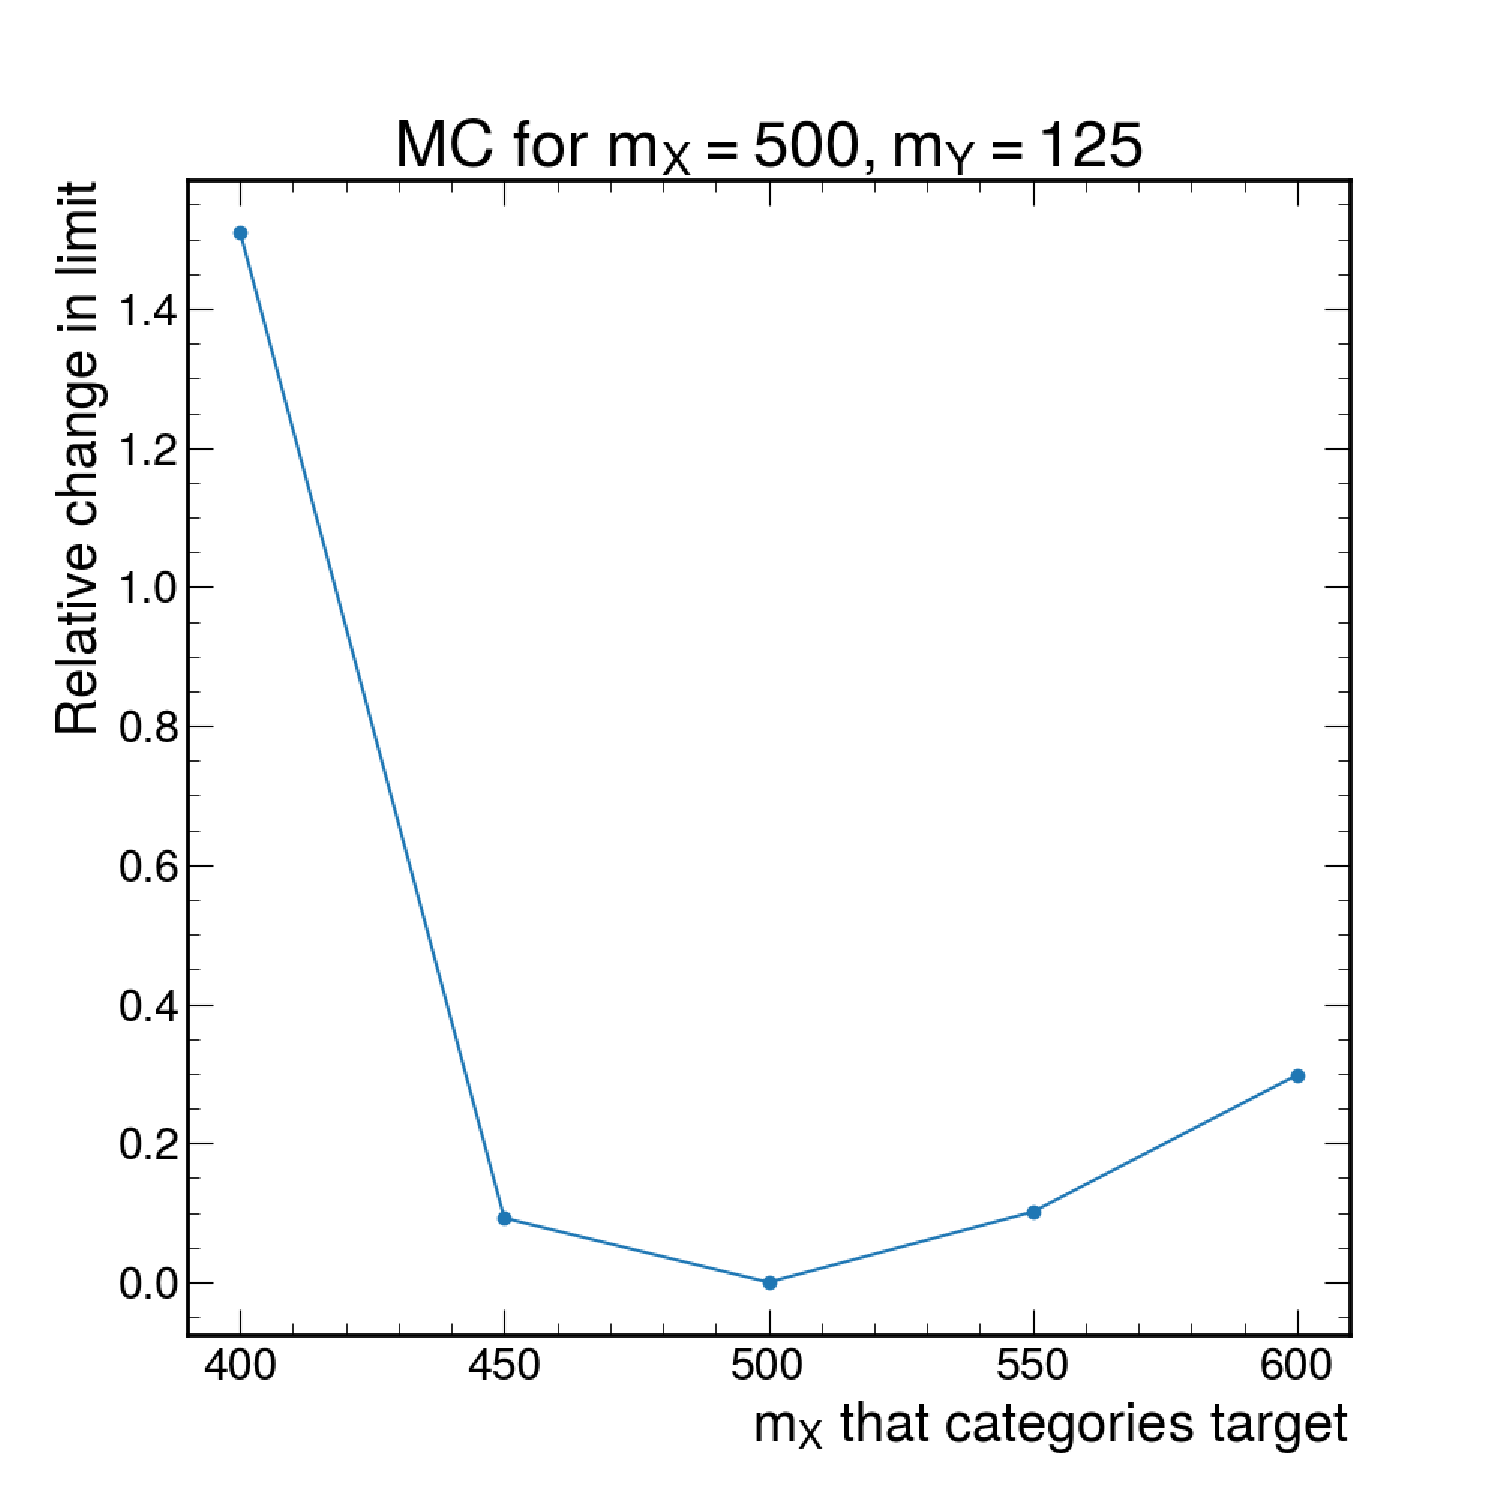
\includegraphics[width=.49\linewidth]{Figures/Dihiggs/results/LimitGranularity/Graviton/mx_500_my_125_mx.pdf}
  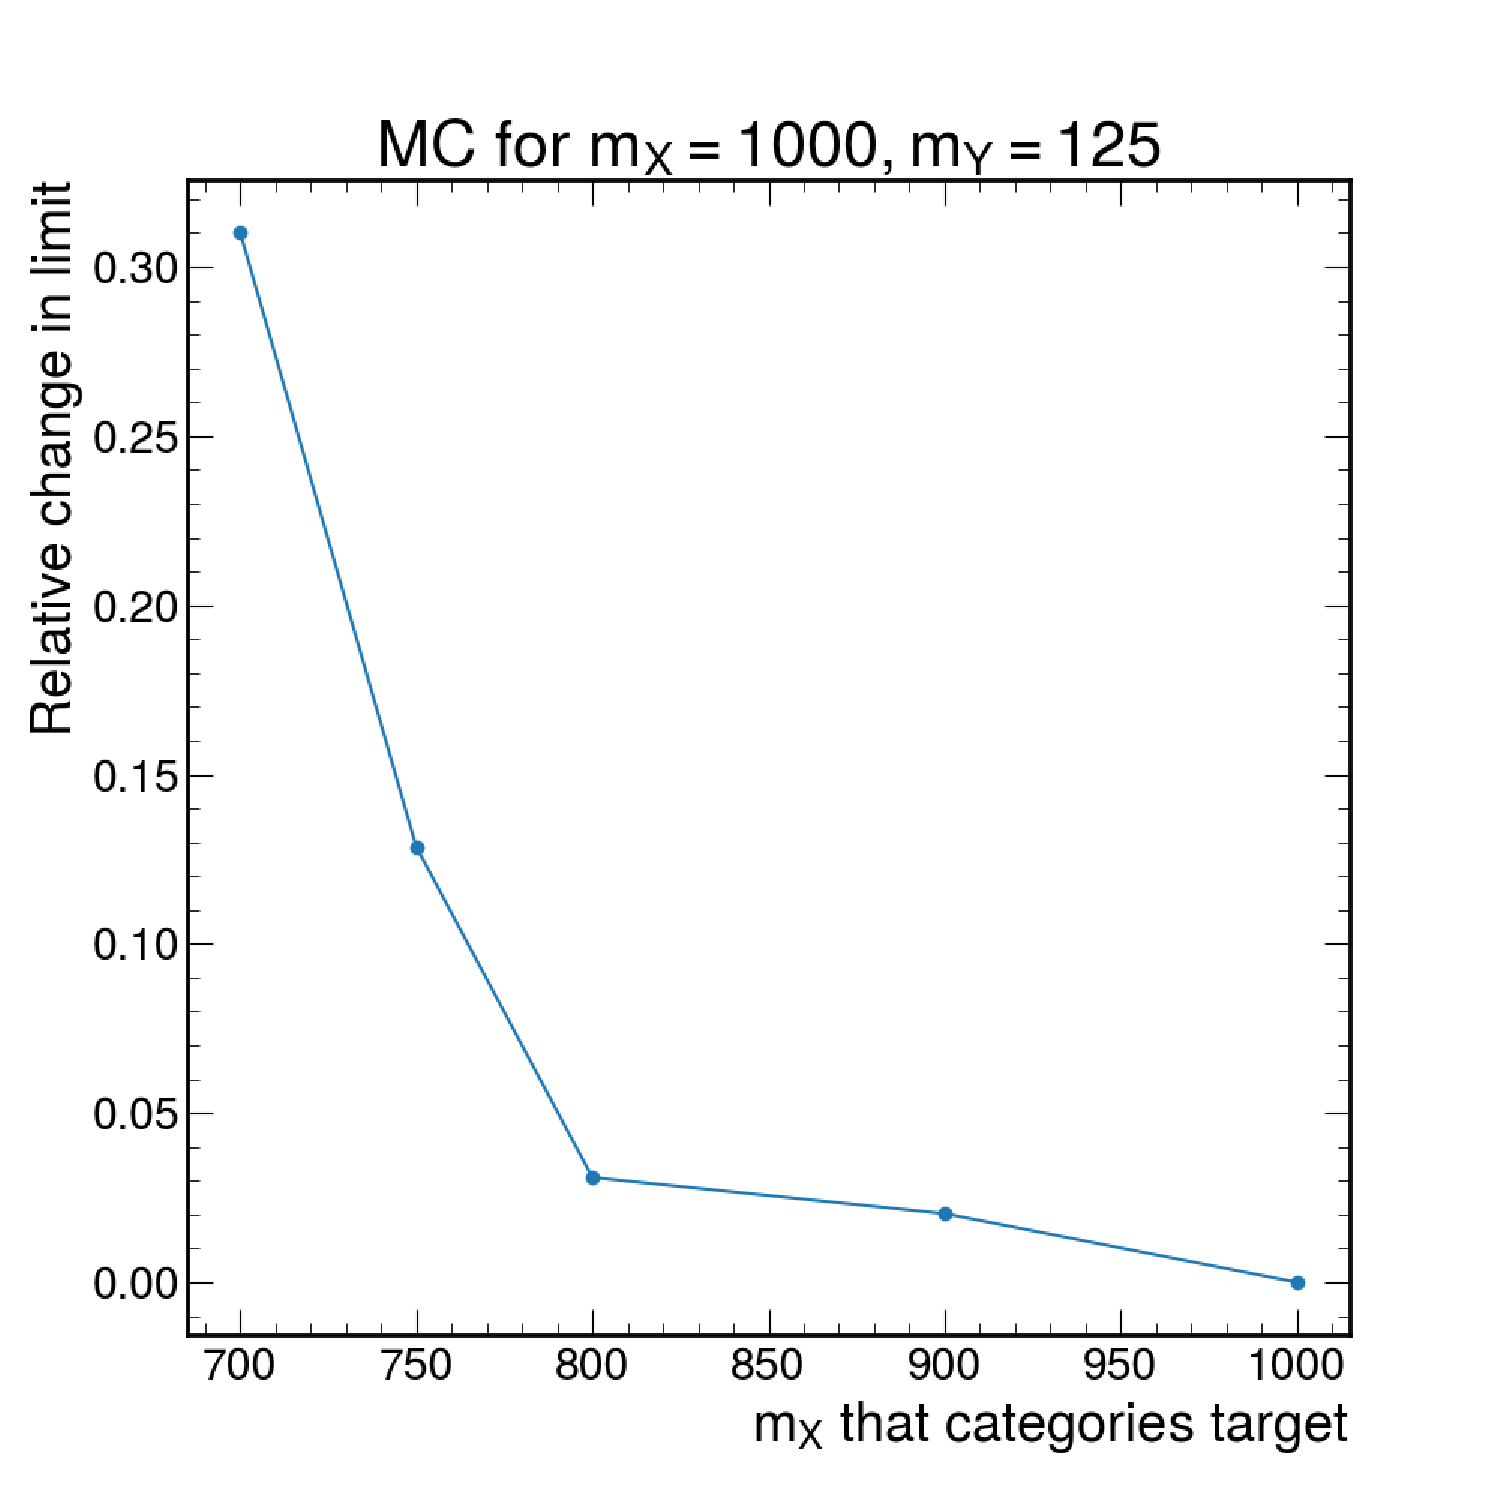
\includegraphics[width=.49\linewidth]{Figures/Dihiggs/results/LimitGranularity/Graviton/mx_1000_my_125_mx.pdf} \\
  \caption[Relative Changes in Expected Upper Limits When Using Categories Not Designed for the Targeted Mass Point]{Relative changes in expected upper limits found for the $\mX=260$ (top-left), 350 (top-right), 500 (bottom-left) and 1000\GeV (bottom-right) \XTwoHH signals when using categories designed to target different mass points. The changes are shown for mass points close to the signal mass, and the change is with respect to the limit found with the categories targeting the signal mass.}\label{fig:limit_granulaity_graviton_changes}
\end{figure}

In the \XHH searches, this is how the granularity of the search is determined, where the number of points added to intervals between nominal mass points is such that the estimated loss in sensitivity is at most 10\%. In the 320--350\GeV example, one could have also considered how the 320\GeV signal performed when using the 350\GeV categories, which could have lead to a greater or lesser worsening in sensitivity than seen when testing the 350\GeV signal with the 320\GeV categories. Therefore, for a given interval, the granularity procedure is performed both ways, and the greatest number of intermediate points determined to be needed is used. The final granularities for the \XZeroHH and \XTwoHH searches were determined separately and are shown in \cref{fig:granularity_xhh}, where 9 intermediate mass points are added to each search. These points are added primarily at low values of \mX where the largest changes in sensitivity are found when using neighbouring categories. At higher values of \mX, such as 500 and 1000\GeV, smaller changes in expected limits are found when using neighbouring categories (\cref{fig:limit_granulaity_graviton_changes}) and therefore fewer intermediate mass points are needed. 

\begin{figure}
  \centering
  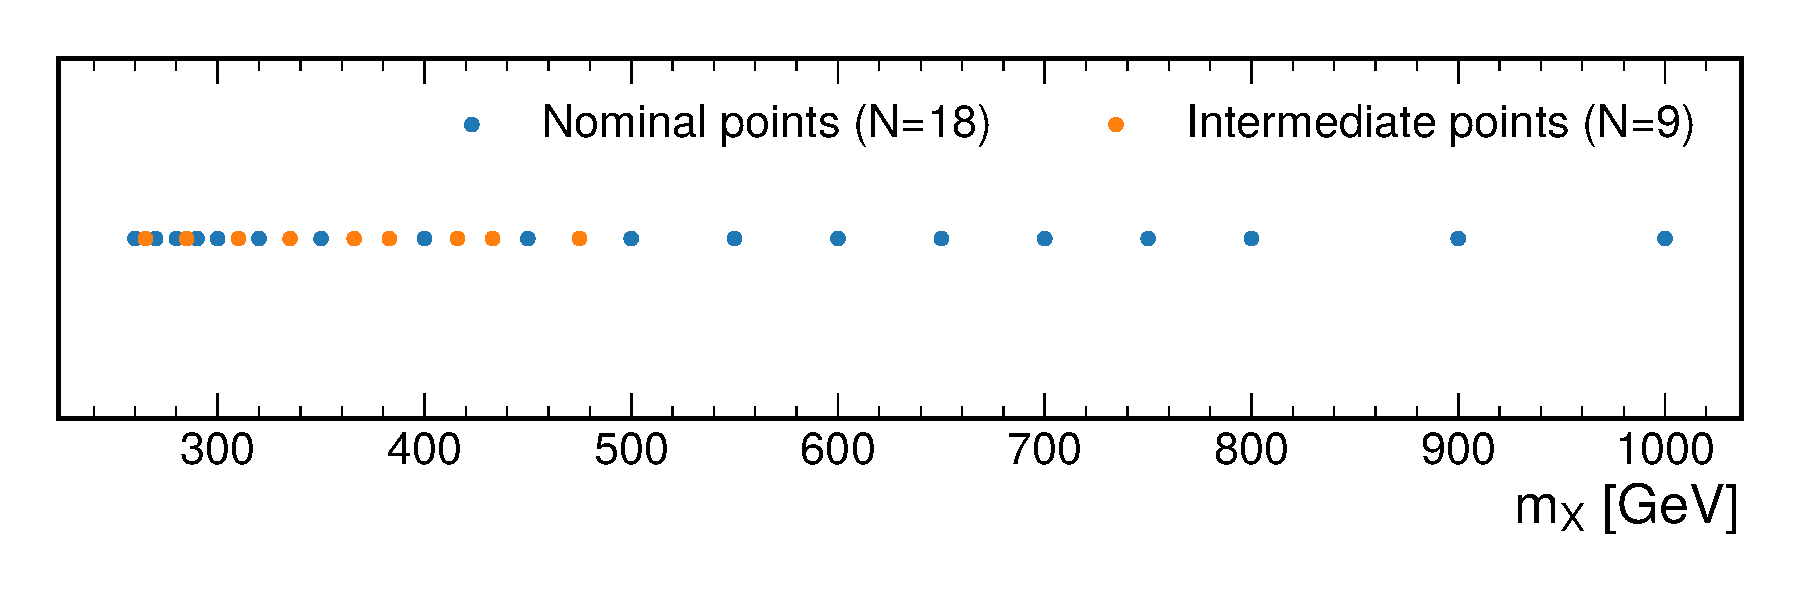
\includegraphics[width=0.8\textwidth]{Figures/Dihiggs/results/LimitGranularity/mass_grid_Radion.pdf}
  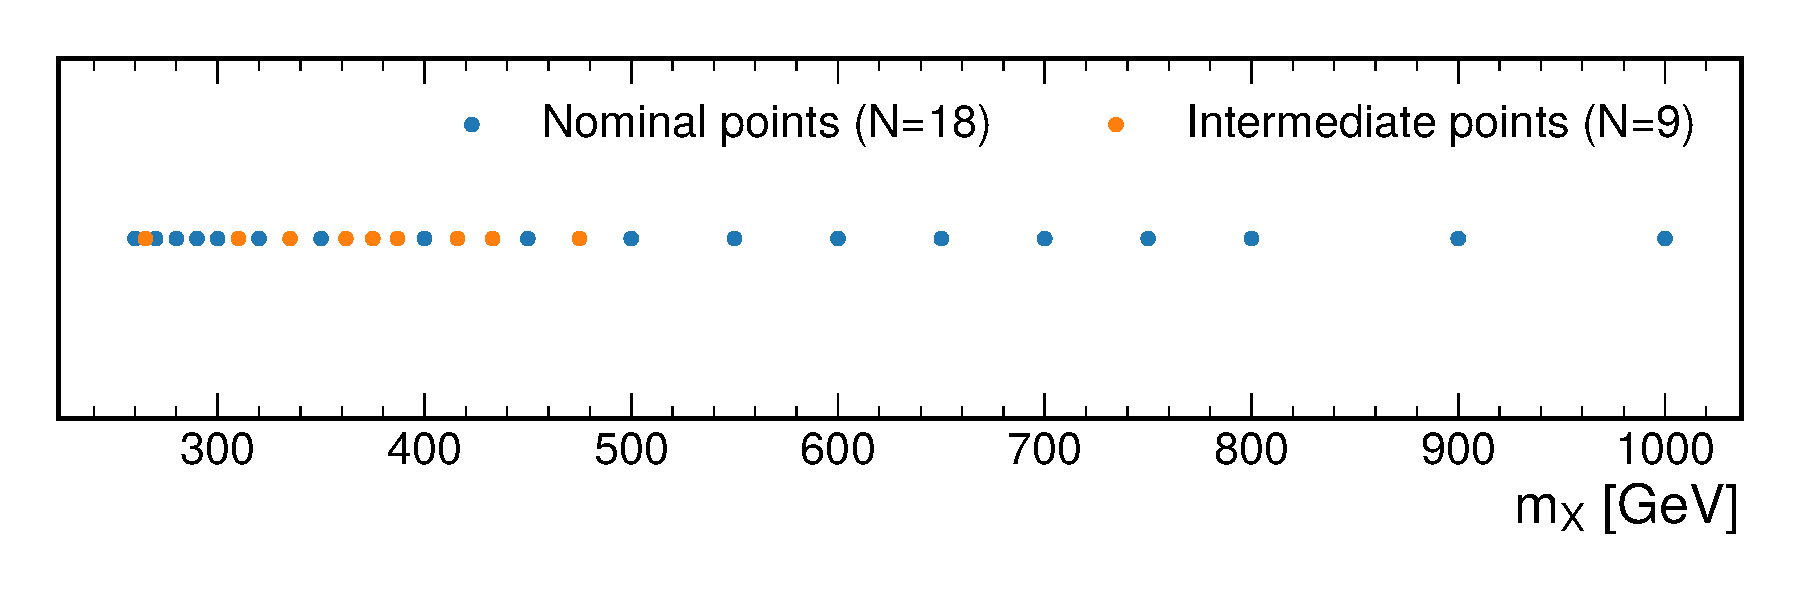
\includegraphics[width=0.8\textwidth]{Figures/Dihiggs/results/LimitGranularity/mass_grid_Graviton.pdf}
  \caption[Search Granularity for the \XHH Searches]{Search granularity for the \XHH searches. Shown are the nominal mass points (blue) and the intermediate mass points (orange) for the \XZeroHH (top) and \XTwoHH (bottom) searches.}\label{fig:granularity_xhh}
\end{figure}

In the \XYH searches, a hollowed-out grid is first formed by applying the same procedure as in the \XHH searches along the \mX and \mY axes independently, in slices of \mY and \mX respectively, where the slices correspond to nominal mass points. Then, the grid must be filled in. For every mass point, $(\mX^i, \mY^j)$, that has an intermediate value of $\mY^j$, the granularity across the \mX axis between $\mX^i$ and the next nominal \mX point is given by the granularity at the previous nominal \mY point. The granularities for the \XYH searches are shown in \cref{fig:granularity_ytt,fig:granularity_low_mass_ygg,fig:granularity_high_mass_ygg}. In the \XYttHgg, low-mass \XYggHtt and high-mass \XYggHtt searches, 310, 93, and 197 intermediate mass points are added. The granularity is again finer at lower \mX, and also at higher \mY where the discrimination between signal and background is more challenging. 

In the $\Ygg$ analyses, an even finer granularity in \mY is defined corresponding to the width of the signal peak in the \mgg distribution. Given that the pNN selection does not change substantially over changes in \mY corresponding to the \mgg resolution, it is not necessary to create dedicated categories for these additional mass points. Instead, the categories defined for the nearest mass point are used. The final number of mass points (nominal plus intermediate) in each search is given in \cref{tab:final_granularity_numbers}. 

\begin{figure}
  \centering
  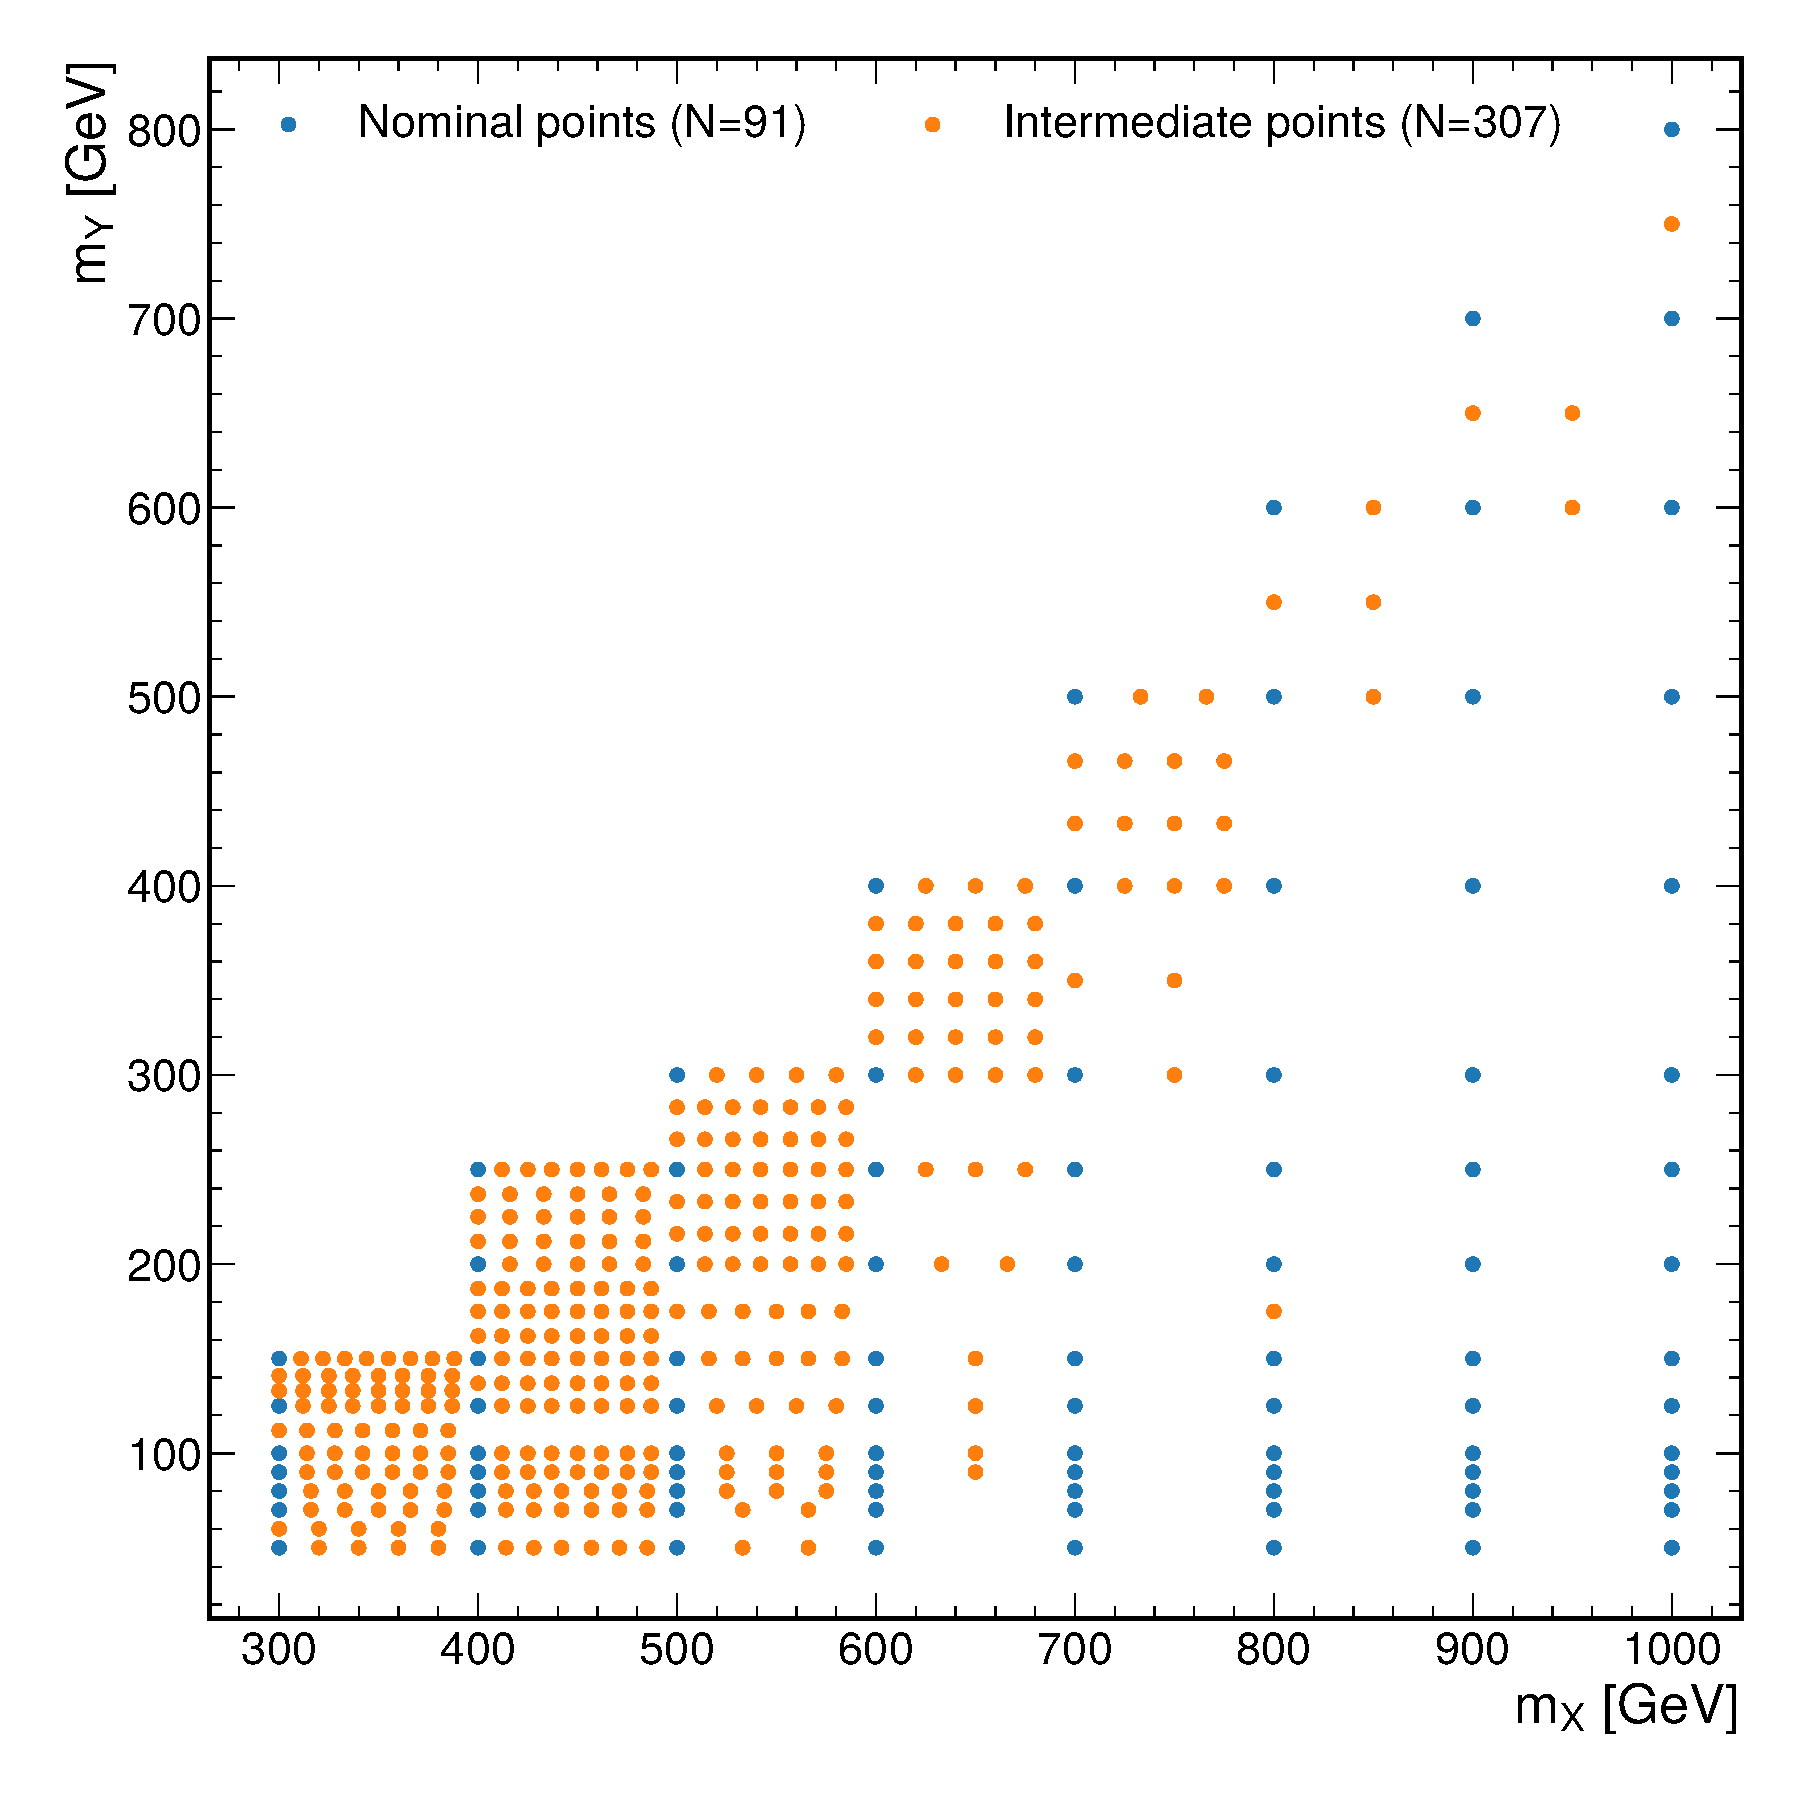
\includegraphics[width=\textwidth]{Figures/Dihiggs/results/LimitGranularity/mass_grid_Y_tautau.pdf}
  \caption[Search Granularity for the \XYttHgg Search]{Search granularity for the \XYttHgg search. Shown are the nominal mass points (blue) and the intermediate mass points (orange).}\label{fig:granularity_ytt}
\end{figure}

\begin{figure}
  \centering
  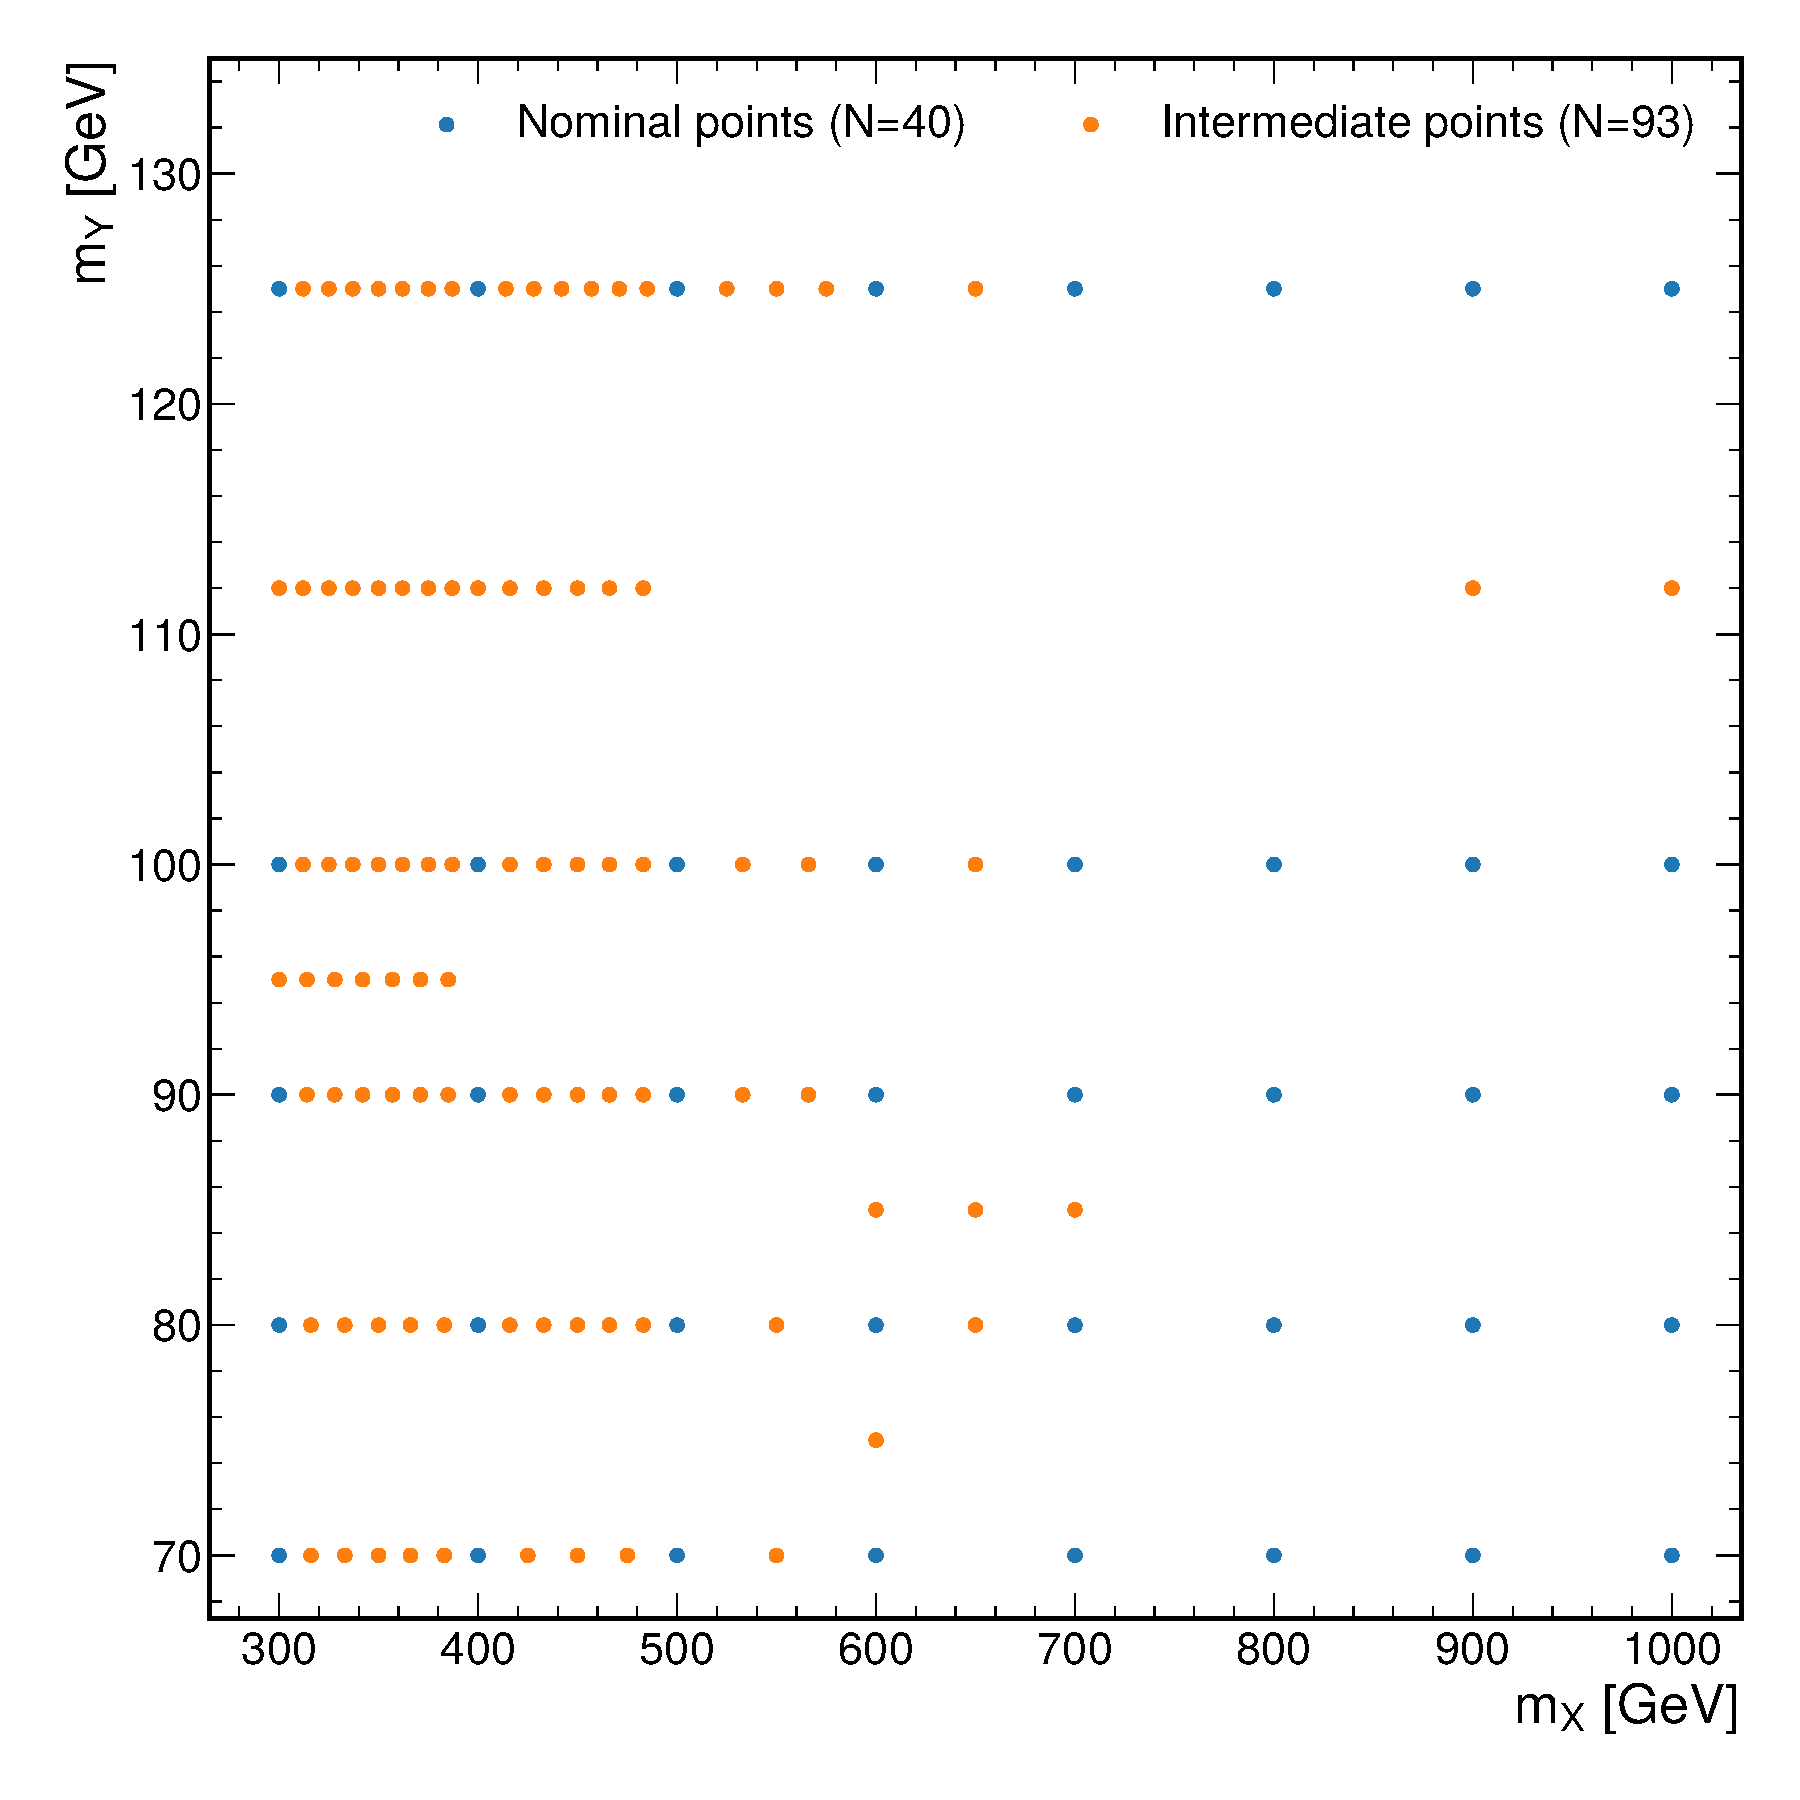
\includegraphics[width=\textwidth]{Figures/Dihiggs/results/LimitGranularity/mass_grid_Y_gg_Low_Mass.pdf}
  \caption[Search Granularity for the Low-Mass \XYggHtt Search]{Search granularity for the low-mass \XYggHtt search. Shown are the nominal mass points (blue) and the intermediate mass points (orange). In addition to the points shown in this plot, searches are also performed at intervals in \mY corresponding to the width of the signal peak in \mgg.}\label{fig:granularity_low_mass_ygg}
\end{figure}

\begin{figure}
  \centering
  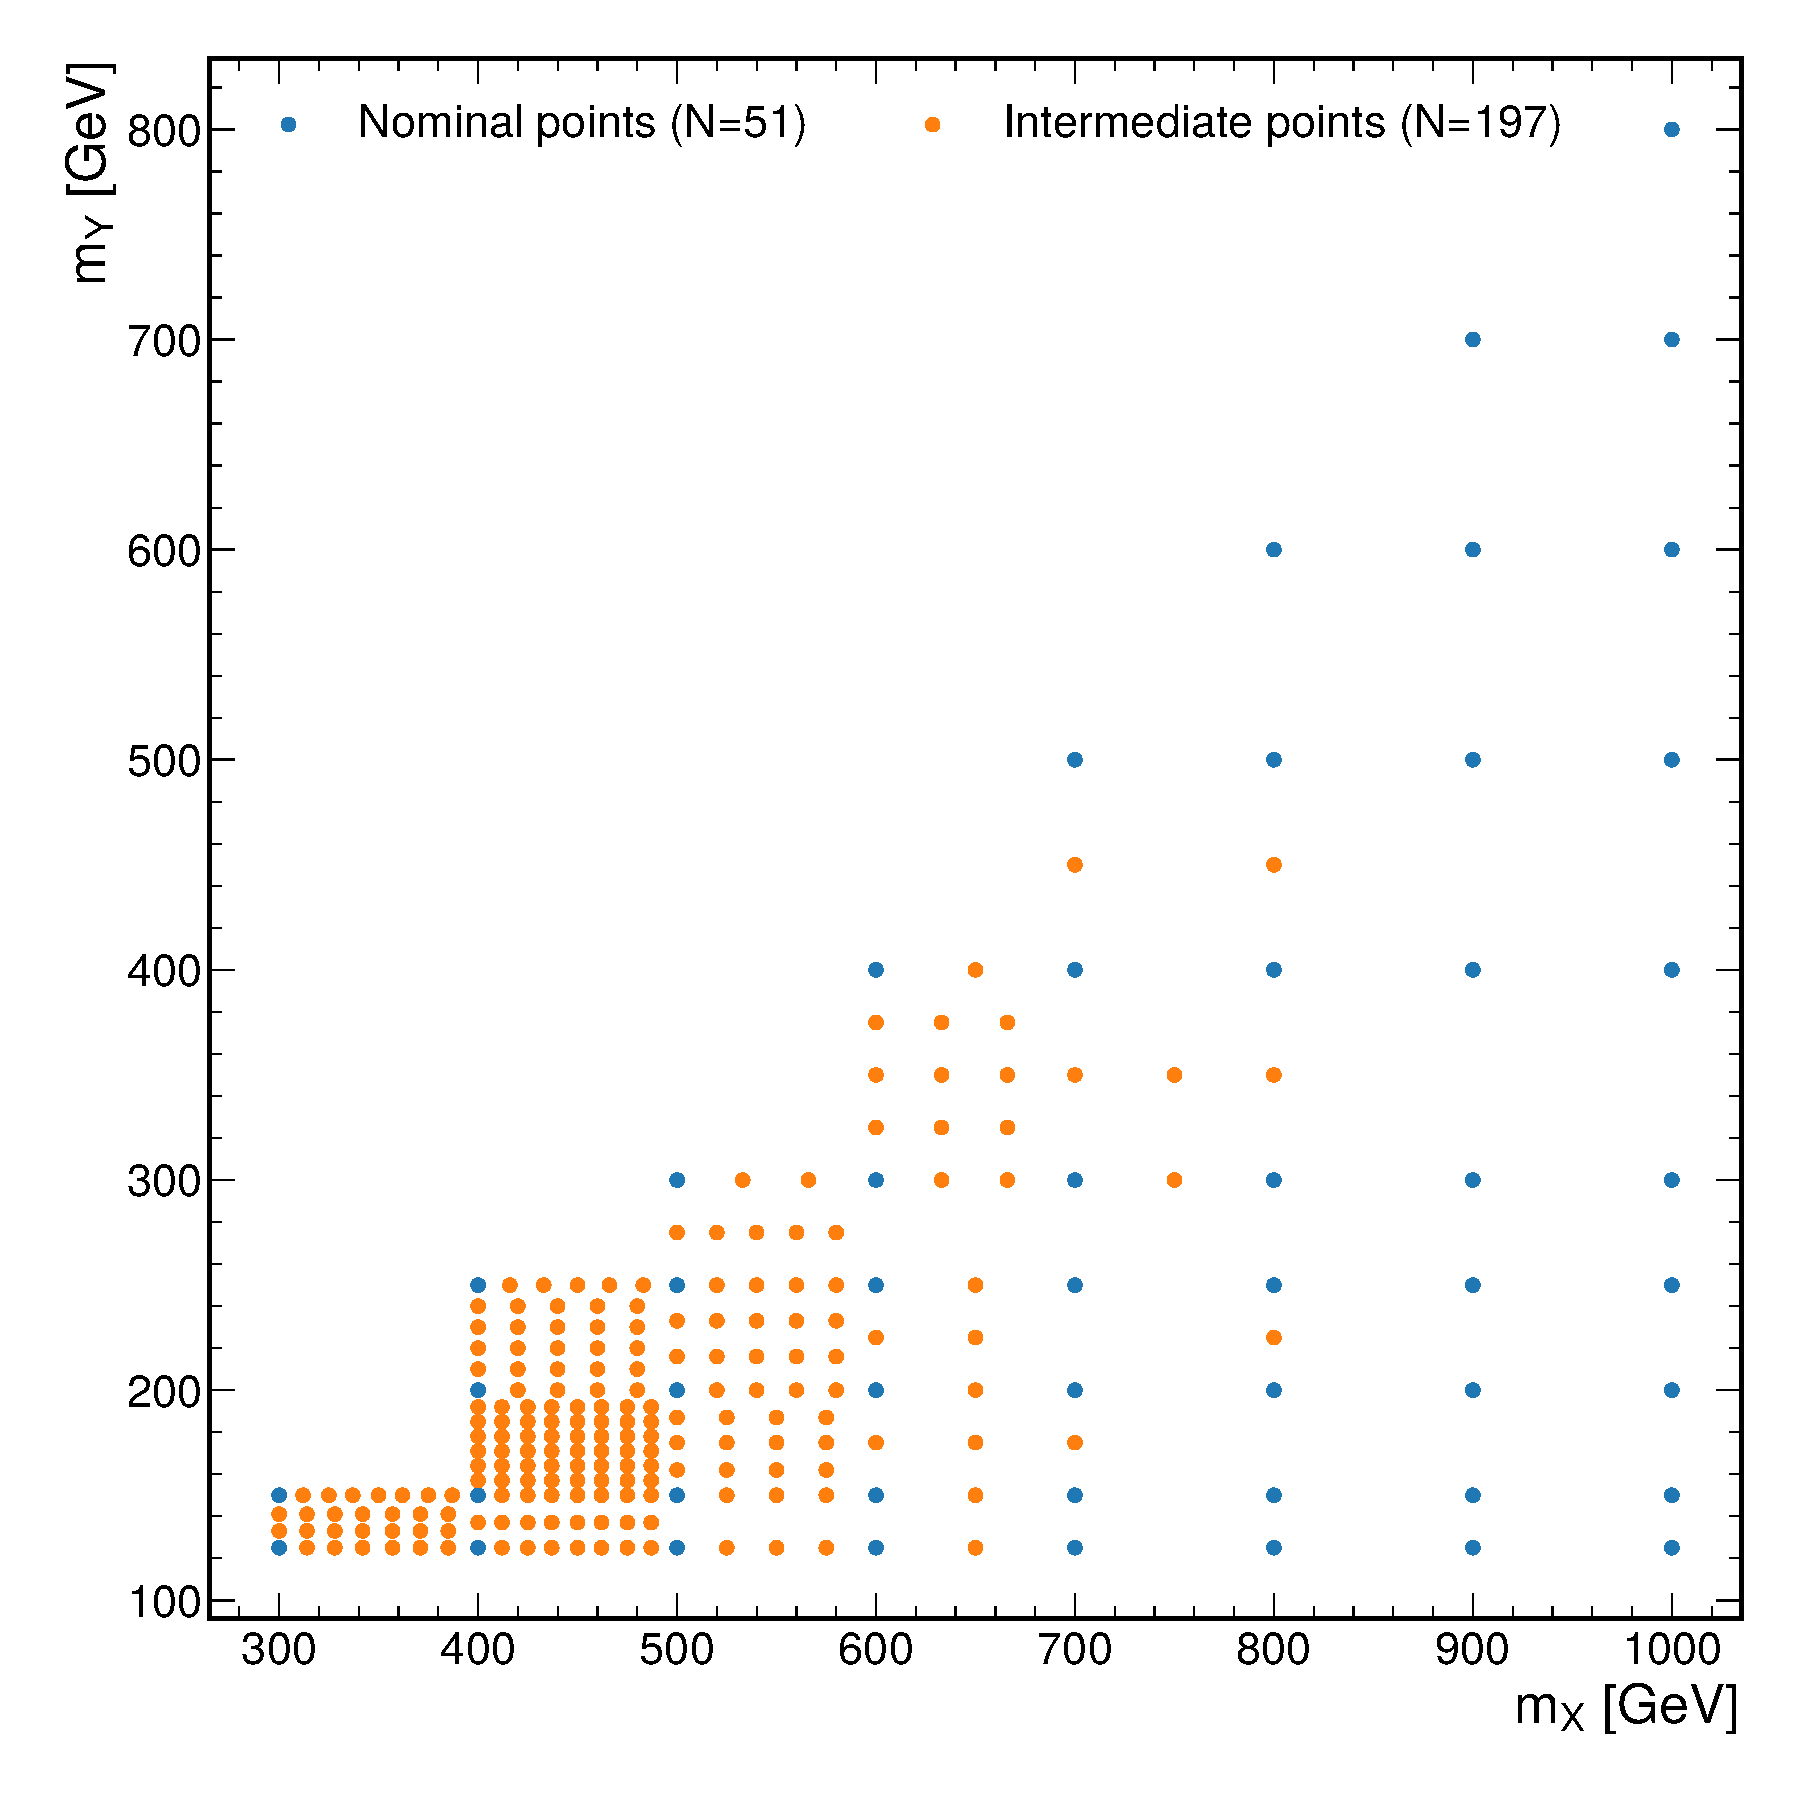
\includegraphics[width=\textwidth]{Figures/Dihiggs/results/LimitGranularity/mass_grid_Y_gg_High_Mass.pdf}
  \caption[Search Granularity for the High-Mass \XYggHtt Search]{Search granularity for the high-mass \XYggHtt search. Shown are the nominal mass points (blue) and the intermediate mass points (orange). In addition to the points shown in this plot, searches are also performed at intervals in \mY corresponding to the width of the signal peak in \mgg.}\label{fig:granularity_high_mass_ygg}
\end{figure}

\begin{table}
  \centering
  \begin{tabular}{cc}
    \toprule
    Search & Number of mass points \\ \midrule
    \XZeroHH & 27 \\
    \XTwoHH & 27 \\
    \XYttHgg & 398 \\
    Low-mass \XYggHtt & 1765 \\
    High-mass \XYggHtt & 2547 \\
    \bottomrule
  \end{tabular}
  \caption[Number of Mass Points in Each Di-Higgs Search]{The total (nominal plus intermediate) mass points considered in each search.}\label{tab:final_granularity_numbers}
\end{table}